\documentclass{article}
\usepackage[spanish]{babel}
% \usepackage{lipsum}
% \usepackage{natbib}
% \usepackage{graphicx}
\newtheorem{art}{Art\' iculo}
\usepackage{titlesec} 
\usepackage{tikz}
\usepackage{fontspec}
\usepackage{xcolor}
\usepackage[a4paper, left=2.5cm,right=2.5cm,top=2.5cm,bottom=2cm]{geometry}
\usepackage{fancyhdr}

\usepackage{eso-pic}
\newcommand\BackgroundPic{%
\put(0,0){%
\parbox[b][\paperheight]{\paperwidth}{%
\vfill
\centering
\includegraphics[width=\paperwidth,height=\paperheight,%
keepaspectratio]{figures/back}%
\vfill
}}}

%------------------Main Font-------------------------
\setmainfont{NotoSansCJKsc}

%C:\Program Files\MiKTeX 2.9\fonts\opentype

%Make sure you have the compiler "XeLaTeX" activated on your settings for your LaTeX document in order to see the font 

%------------------Color Set--------------------------
\definecolor{LightBlue}{RGB}{250, 193, 6}
\definecolor{DarkBlue}{RGB}{138, 109, 28}
\definecolor{LightGray}{gray}{.94}
\definecolor{DarkGray}{gray}{.172}
\definecolor{Orange}{RGB}{229, 133, 3}
\definecolor{MediumBlue}{RGB}{184, 146, 40}

%------------------Section Default Setting-------------
\titleformat*{\section}{\color{DarkBlue}\normalfont\bfseries\Huge}
\titleformat*{\subsection}{\color{LightBlue}\normalfont\bfseries\Large}
\titleformat*{\subsubsection}{\color{MediumBlue}\normalfont\bfseries\LARGE}

%-------------------Section Numbers Removal------------
\setcounter{secnumdepth}{0}


%-------------------------Header & Footer------------------------

\pagestyle{fancy}
\fancyhf{}
\fancyhead[L]{
\begin{tikzpicture}[remember picture,overlay] \node[anchor=north west, yshift=1.5mm, xshift=-1.5mm] at (current page.north west) {\includegraphics[height=25mm]{figures/header_corner.png}};
\end{tikzpicture}
}
\fancyfoot[C]{
\begin{tikzpicture}[remember picture,overlay] \node[anchor=south east, yshift=-1.5mm, xshift=1.5mm] at (current page.south east) {\includegraphics[width=210mm]{figures/banner.png}};
\end{tikzpicture}
\textcolor{LightGray}{\thepage}
}

%------------------Document----------------------------

\begin{document}
\AddToShipoutPicture*{\BackgroundPic}
\begin{titlepage}
\newcommand{\HRule}{\rule{\linewidth}{0.5mm}} 
\center
{\Huge \bfseries Octava Semana \\ Electrónica 2019} \\[1cm]
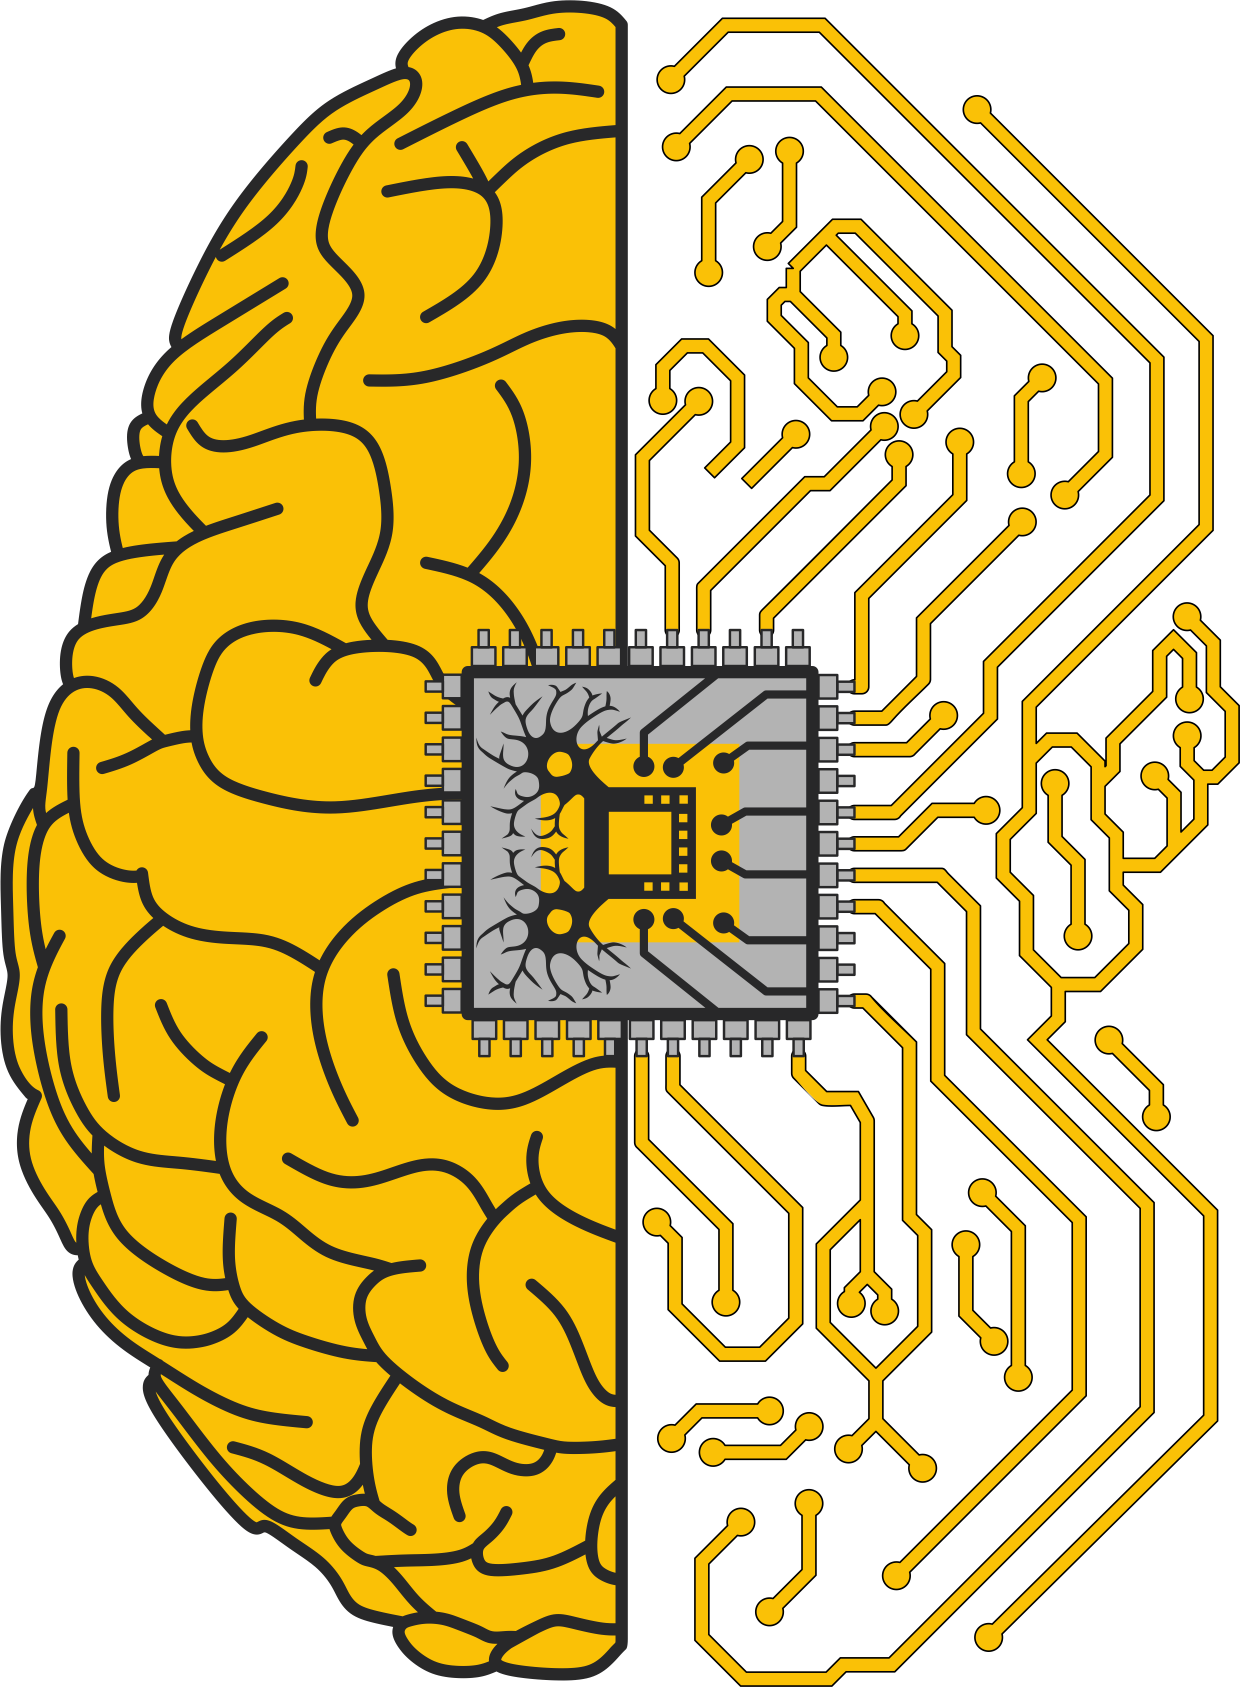
\includegraphics[width=6cm]{figures/Li-UNSAAC}\\[1cm]
\textsc{\LARGE  Universidad Nacional de San \\[0.2cm] Antonio Abad del Cusco}\\[0.4cm] 
\textsc{\Large Facultad de Ingeniería Eléctrica, \\ Electrónica, Informática y Mecánica}\\[0.4cm] 
\textsc{\large Escuela Profesional de Ingeniería Electrónica}\\[0.4cm]
\HRule \\[0.4cm]
{ \huge \bfseries Concurso de Mascota}\\[0.3cm] 
\HRule \\[1.5cm]
\today
\end{titlepage}



\newpage
\noindent
\normalfont

\section{PRESENTACIÓN}
\normalfont

La Universidad Nacional de San Antonio Abad del Cusco (UNSAAC), a través de la Escuela Profesional de Ingeniería Electrónica, en cumplimiento de las normas que rigen la investigación, con el objetivo de difusión y promoción de Investigación en tecnología de actualidad; organizado por la \textbf{VIII Semana Electrónica UNSAAC} presenta el \textbf{Concurso de Mascotas - Ingeniería Electrónica UNSAAC 2019}, el cual hace un extenso llamado a estudiantes, centros de investigación, circulos de investigación, circulos de estudio de la UNSAAC para formar parte de este concurso que hará que su propuesta quede por mucho tiempo como símbolo de la Escuela Profesional dando cara en diferentes eventos tanto recreativos como académicos.

\section{ORGANIZACIÓN}

La Universidad Nacional de San Antonio Abad del Cusco a través de la Escuela Profesional de Ingeniería Electrónica.

\section{OBJETIVOS}

Promover e incentivar estudiantes de la Escuela Profesinal de Ingeniería Electrónica UNSAAC a presentar una mascota que será simbolo de todos los estudiantes y toda la Escuela Profesional en diferentes eventos.

\section{LINEAMIENTOS DE CONVOCATORIA}

Los trabajos que se aceptarán serán aquellos que cumplan alguna de los siguientes tipos de presentación.


\begin{tabular}{|p{5cm}|p{10cm}|}
\hline
\textbf{Lineamiento} & \textbf{Característica} \\ \hline
Diseño propio digital & Este deberá estar entera o parcialmente diseñado con algún software de diseño como Photoshop, Corel Draw, Ilustrator, etc. El personaje de creación propia o de terceros deberá exportarse en una imagen de extensión \texttt{.pdf}, \texttt{.jpg}, \texttt{.png} en tamaño A4 (disposición vertical) a todo color. Se recomienda usar la extensión de \texttt{.pdf} en fondo blanco o algún otro que no quite relevancia al objeto en concurso.\\ \hline
Diseño a color en papel o algún lienzo & Este trabajo deberá estar escaneado en un archivo de extensión \texttt{.pdf} de tamaño A4 (disposición vertical). Se recomienda usar fondo blanco a fin de no quitar protagonismo al objeto en concurso.  \\ \hline
Imagen de autoría de terceros &  Esta imagen que es de autoría de terceros puede ser diseñada en papel o diseño digital, en tal caso se deberá incluir el origen de la imagen en un pie de página para reconocer su autoría. En el caso de sacar una imagen de internet, incluir la dirección web de esta imagen e incluirla en el pié de página. Se recomienda usar un fondo blanco o algún otro que no quite protagonismo al objeto en concurso. También se tendrá que presentar en un archivo de extensión \texttt{.pdf} de tamaño A4 (disposición vertical).  \\ \hline
\end{tabular}

\section{ESPECIFICACIONES DE LAS PROPUESTAS}
La propuesta de mascota deberá ir acompañado de los aneños 1 y 2 de manera obligatoria, y del anexo 3 siempre y cuando sea autor completo de la obra.
 
\subsection{Especificaciones}
 
 Se recomienda que el objeto del concurso ocupe un area considerable en la hoja A4 a fín de que toda la escuela profesional pueda apreciar cada trabajo para una justa elección.
 
 Además de las características señaladas en los Lineamientos de Convotaroria, el participante o grupo de estudiantes deberán adjuntar lo siguiente:
 
 \begin{enumerate}
 \item \textbf{Simbolismo}, la mascota que cada participante propondrá debe tener algun tipo de sustento, haciendo énfasis de las razones por las que debería representar a la Escuela Profesional de Ingeniería Electrónica.
 \item \textbf{Atractivo}, el participante deberá sustentar la razón por la cual su propuesta es atractiva, la razón por la que cree que será querida y aceptada por toda la Escuela Profesional de Ingeniería Electrónica. Estas características pueden ser el color, el morfimo, o alguna ota característica que el participante vea por conveniente.
 \item \textbf{Palabras finales}, el participante puede agregar lo que vea por conveniente, como algún agradecimiento, o alguna otra razón por la cual su propuesta debería ser la elegida.
 \end{enumerate}
 
 Lo señalado en los item 1, 2 y 3 deberan ir en párrafos separados y deberá llevar el nombre de la mascota en concurso como título. Todo el contenido no debe exceder 1 hoja. Usar la fuenre \textbf{Arial, Calibri} o \textbf{Times New Roman} de tamaño 12 de color negro, con márgenes superios, inferior, derecha e izquierda no menores de 2cm. 
 

\section{PARTICIPANTES}

\begin{itemize}
\item Estudiantes de la Escuela Profesional de Ingeniería Electrónica de la Universidad Nacional de San Antonio Abad del Cusco.
\item Centros de Investigación, Circulos de Investigación y Estudio de la Universidad Nacional de San Antonio Abad del Cusco.
\end{itemize}

\subsection{Modalidad}

\begin{itemize}
\item Participación individual.
\item Participación grupal con 3 integrantes como máximo.
\end{itemize}

\section{RECONOCIMIENTOS}

Los resultados de la competencia son inapelable. El trabajo ganador recibirá un reconocmiento e incentivo por parte de la Escuela profesional de Ingeniería Electrónica a través de los ingenieros de la misma y recibirá certificación de ganador.

\section{ETAPAS}

\begin{tabular}{|p{8cm}|p{8cm}|}
\hline
\textbf{ETAPA} &  \textbf{REQUSITOS} \\ \hline
Convocatoria por la Escuela Profesional de Ingeniería Electrónica 
& Estudiantes, Centros de Investigación, Circulos de Investigación y Estudio de la Universidad Nacional de San Antonio Abad del Cusco. \\ \hline

Inscripciones de Trabajos del \textbf{14 de noviembre} hasta el \textbf{20 de noviembre} hastas la media noche enviando su trabajo a circae.unsaac@gmail.com & 
Llenar los formatos anexados en estas bases (Anexo 1, Anexo 2 de manera obligatoria y opcional Anexo 3). \\ \hline

Publicación de propuestas \textbf{21 de noviembre} 
& La comisión organizadora publicará las propuestas en la página Oficial de La escuela Profesional de Ingeniería Electrónica \texttt{https://www.facebook.com/Ingeniería-Electrónica-Unsaac-100140831455046/}, también se pegará en pmresiones a color en lugares estratégicos del Pabell´pon de Ingeniería Electrónica. \\ \hline

Elección de la Mascota \textbf{22 de noviembre}& 
Sellevará durante el transcurso del día. Los Circulos de Estudio, Centros de Investigación, Centro Federado y demás organizaciónes que pertenecen a la Escuela Profesional de Ingeniería Electrónica deberán ejercer su voto de manera obligatoria. Cada organización deberá hacer su elección en el modo que ellos vean conveniente, pero tendrán que presentar un sustento por escrito, con la cantidad de votos por cada propuesta, y deberá ir firmada por su representante. Los estudiantes que no estén en alguna organización ligada a la Escuela Profesional, podrán ejercer su voto a través del centro federado, este ente se encargará de la organización y ejecusión de las elecciones para estos estudiantes. El voto de cada estudiante es única, y es muy importante, por que este proceso llevará a un ganador, y será la representación de todos. Los ingenieros de la Escuela Profesional de Ingeniería Electrónica de la UNSAAC también tendrán opción a votar y será de manera individual. EL voto de cada ingeniero equivale a 10 votos de estudiante, esto por que somos más de 300 estudiantes y los ingenieros son un poco más de 10. El proceso de votación de los ingenieros estará encargada por una comisión y de igual manera, deberán presentar un sustento por escrito, con la cantidad de votos por cada propuesta, y deberá ir firmada por cada ingeniero sufragante.\\ \hline

Declaración de ganador se dará la noche del \textbf{22 de noviembre}
& Luego del conteo de vot, se hará la publicación por las redes sociales y se publicará en los murales de la Escuela Profesional mostrando gráficos estadísticos del resultado final.\\ \hline

La Mascota de Ingeiería Electrónica & 
Se hará la confección en el transcurso de la semana siguiente a la elección. y se pondrá una marca o nombre si el participante ganador así lo desea.\\ \hline

Presentación de la Mascota & 
Se hará en la \textbf{VIII Semana Electrónica UNSAAC 2019} y la persona que interprete la mascota será por voluntad de cualquier etudiante, o el participante ganador si así lo desea. \\ \hline

\end{tabular}

\textbf{Cualquier aspecto que no se haya considerado en las bases, será resuelto por la comisión 
organizadora de la VIII Semana Electrónica UNSAAC 2019}

\newpage
{\center
{\Huge \bfseries Octava Semana Electrónica 2019} \\ [0.4cm]
\textsc{\LARGE  Universidad Nacional de San Antonio Abad del Cusco}\\[0.4cm] 
\textsc{\Large Facultad de Ingeniería Eléctrica, Electrónica, Informática y Mecánica}\\[0.4cm] 
\textsc{\large Escuela Profesional de Ingeniería Electrónica}\\[0.4cm]
{ \bfseries Anexo1 - Datos Generales}}

\subsubsection{Nombre de la Mascota}

.....................................................................................................................................................................

.....................................................................................................................................................................

.....................................................................................................................................................................

.....................................................................................................................................................................


\subsubsection{Datos Generales}

\begin{tabular}{|p{5cm}|p{10cm}|}
\hline
Nombres & \\ \hline
Apellidos & \\ \hline
DNI & \\ \hline
Código & \\ \hline
Sexo & \\ \hline
E-mail & \\ \hline
Numero de teléfono movil & \\ \hline
Dirección & \\ \hline
Escuela Profesional & \\ \hline
Número de participante del Equipo & \\ \hline
\end{tabular}

\begin{figure}[hbtp]
\centering
\includegraphics[width = 6cm]{IMAGENES/firma.jpg}
\caption{Huella digital, firma con nombre completo y DNI}
\end{figure}

\newpage
{\center
{\Huge \bfseries Octava Semana Electrónica 2019} \\ [0.4cm]
\textsc{\LARGE  Universidad Nacional de San Antonio Abad del Cusco}\\[0.4cm] 
\textsc{\Large Facultad de Ingeniería Eléctrica, Electrónica, Informática y Mecánica}\\[0.4cm] 
\textsc{\large Escuela Profesional de Ingeniería Electrónica}\\[0.4cm]
{ \bfseries Anexo2 - Formulario de Inscripción}}

\subsubsection{Nombre de la Mascota}

.....................................................................................................................................................................

.....................................................................................................................................................................

.....................................................................................................................................................................

.....................................................................................................................................................................



\subsubsection{Resumen del Significado de La Mascota}

.....................................................................................................................................................................

.....................................................................................................................................................................

.....................................................................................................................................................................

.....................................................................................................................................................................

.....................................................................................................................................................................

.....................................................................................................................................................................

.....................................................................................................................................................................

.....................................................................................................................................................................

.....................................................................................................................................................................

.....................................................................................................................................................................

.....................................................................................................................................................................

.....................................................................................................................................................................

.....................................................................................................................................................................

.....................................................................................................................................................................


\textbf{Al firmar el documento, acepta los términos y condiciones de las bases.}

\begin{figure}[hbtp]
\centering
\includegraphics[width = 6cm]{IMAGENES/firma.jpg}
\caption{Huella digital, firma con nombre completo y DNI}
\end{figure}

\newpage
{\center
{\Huge \bfseries Octava Semana Electrónica 2019} \\ [0.4cm]
\textsc{\LARGE  Universidad Nacional de San Antonio Abad del Cusco}\\[0.4cm] 
\textsc{\Large Facultad de Ingeniería Eléctrica, Electrónica, Informática y Mecánica}\\[0.4cm] 
\textsc{\large Escuela Profesional de Ingeniería Electrónica}\\[0.4cm]
{ \bfseries Anexo3 - Declaración Jurada}}

\subsubsection{DECLARACIÓN JURADA DE NO PLAGIO}

Yo, ........................................................................................................................................, con DNI Número 
......................, participante del \textbf{Concurso de Mascota de la Escuela Profesional de Ingeniería Electrónica UNSAAC} presentado en la \textbf{VIII Semana Electrónica UNSAAC 2019}, con la Mascota de nombre :

.....................................................................................................................................................................

.....................................................................................................................................................................

.....................................................................................................................................................................


Declaro bajo juramento que: 

\begin{itemize}
\item El trabajo a presentarse en la presente convocatoria, es de mi autoría. 
\item El proyecto no ha sido 
plagiado total ni parcialmente. 
\item El proyecto no ha sido autoplagiado, es decir no ha sido presentado ni publicado anteriormente. De 
identificarse fraude (datos falsos), plagio (información sin citar autores), autoplagio (presentar como 
nuevo algún trabajo que ya ha sido presentado), piratería (uso ilegal de 
información ajena) o falsificación (representar falsamente las ideas de otros), asumo las consecuencias 
y sanciones que de mi acción se deriven, sometiéndome a las normas de la Universidad así como a la 
normatividad nacional competente.
\end{itemize}

Cusco, .......... de noviembre del 2019




\textbf{Al firmar el documento, acepta los términos y condiciones de las bases.}

\begin{figure}[hbtp]
\centering
\includegraphics[width = 6cm]{IMAGENES/firma.jpg}
\caption{Huella digital, firma con nombre completo y DNI. }
\end{figure}

Adjuntar Copia de DNI



\end{document}
